\documentclass[12pt, t]{beamer}

\usepackage{graphicx}
\usepackage{amsmath}
\usepackage{setspace}
\usepackage{float} 
\usepackage{multido}
\usepackage{multirow}
\usepackage{array}
\usepackage{enumerate}
\usepackage{booktabs}
\usepackage{indentfirst} 
\usepackage[style=mla]{biblatex}
\usepackage{subcaption}
\usepackage{hyperref}
\usepackage{textpos}

\makeatletter
\let\@@magyar@captionfix\relax
\makeatother

\definecolor{Turquoise3}{RGB}{0, 134, 139}
\renewcommand{\emph}[1]{{\color{Turquoise3}\textsl{#1}}}
\newcommand{\C}{\mathbb{C}} \newcommand{\F}{\mathbb{F}} \newcommand{\R}{\mathbb{R}} \newcommand{\Q}{\mathbb{Q}}
\newcommand{\N}{\mathbb{N}}
\newcommand{\myseries}[2]{$#1_1,#1_2,\dots,#1_#2$}
\newcommand{\nullspace}{~\\[15pt]}
\newcommand{\remark}{\textbf{Remark: }}
\newcommand{\scp}[2]{\langle\,#1\,,\,#2\,\rangle} \newcommand{\scpp}{\langle\,\cdot\,,\,\cdot\,\rangle}


\usetheme{Madrid}
\setbeamertemplate{navigation symbols}{}

\addtobeamertemplate{frametitle}{}{
\begin{textblock*}{100mm}(0.85\textwidth,-1cm)

\includegraphics[height=1cm]{logo.png}
\end{textblock*}}

\definecolor{themecolor}{RGB}{25,25,112} 

\usecolortheme[named=themecolor]{structure}

\setbeamertemplate{items}[default]

\hypersetup{
    colorlinks=true,
    linkcolor=themecolor,
    filecolor=themecolor,      
    urlcolor=themecolor,
    citecolor=themecolor,
}

\title{VV285 RC Part II}
\subtitle{\textbf{Elements of Linear Algebra}\\``Linear Algebra!"}
\institute[UM-SJTU JI]{Univerity of Michigan-Shanghai Jiao Tong University Joint Institute}
\author{Yiwen Tu}

\begin{document}

\begin{frame}
    \titlepage
    \begin{center}
        
\includegraphics[height=2cm]{logo2.png}
    \end{center}
\end{frame}

\begin{frame}
    \frametitle{Systens of Equations}
    \begin{center}
        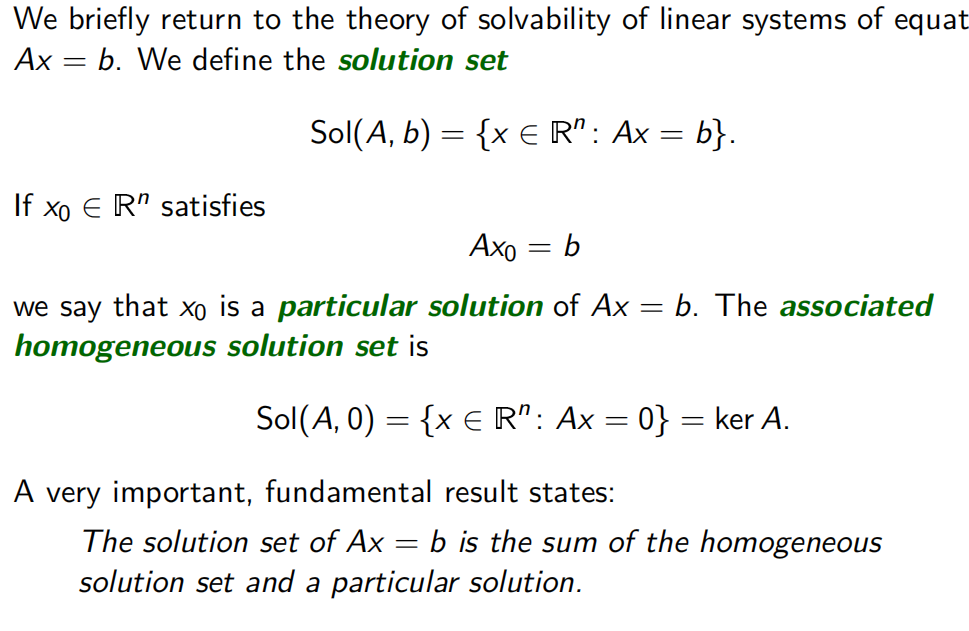
\includegraphics[width=\textwidth]{0}
    \end{center}
\end{frame}

\begin{frame}
    \frametitle{Systens of Equations}
    \begin{center}
        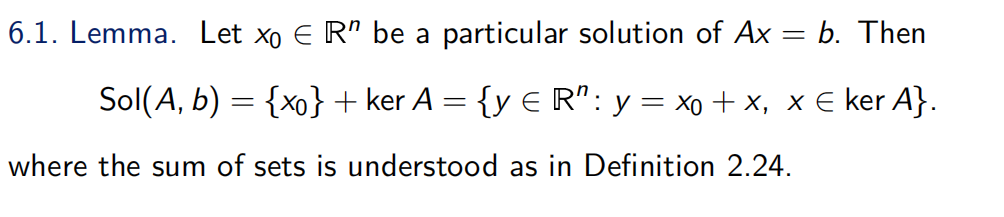
\includegraphics[width=\textwidth]{2}
    \end{center}
\end{frame}

\begin{frame}
    \frametitle{Systens of Equations}
    \begin{center}
        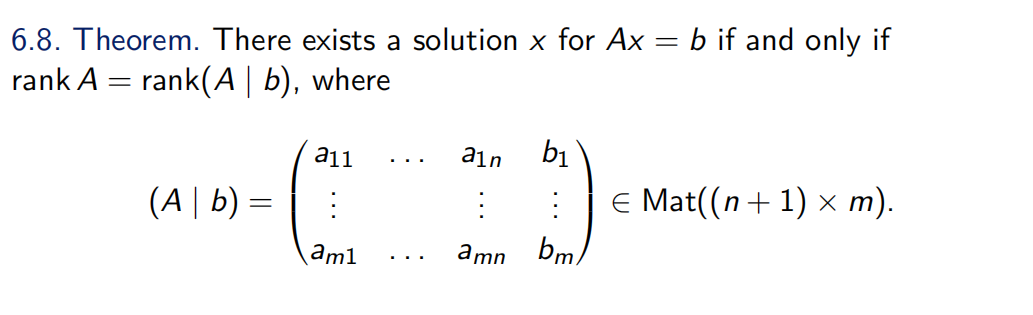
\includegraphics[width=\textwidth]{3}
    \end{center}
\end{frame}

\begin{frame}
    \frametitle{Systens of Equations}
    \begin{center}
        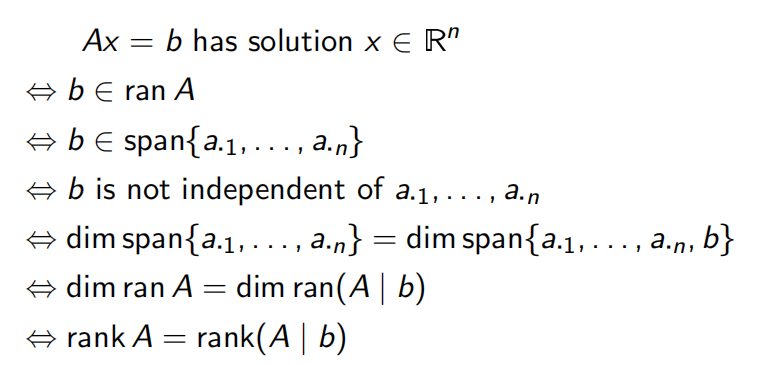
\includegraphics[width=\textwidth]{4}
    \end{center}
\end{frame}

\begin{frame}
    \frametitle{Systens of Equations}
    \begin{center}
        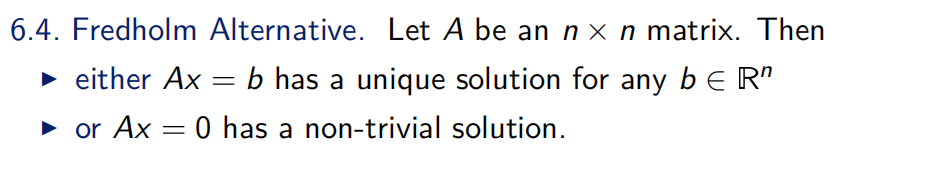
\includegraphics[width=\textwidth]{7}
    \end{center}
\end{frame}

\begin{frame}
    \frametitle{Systens of Equations}
    \begin{center}
        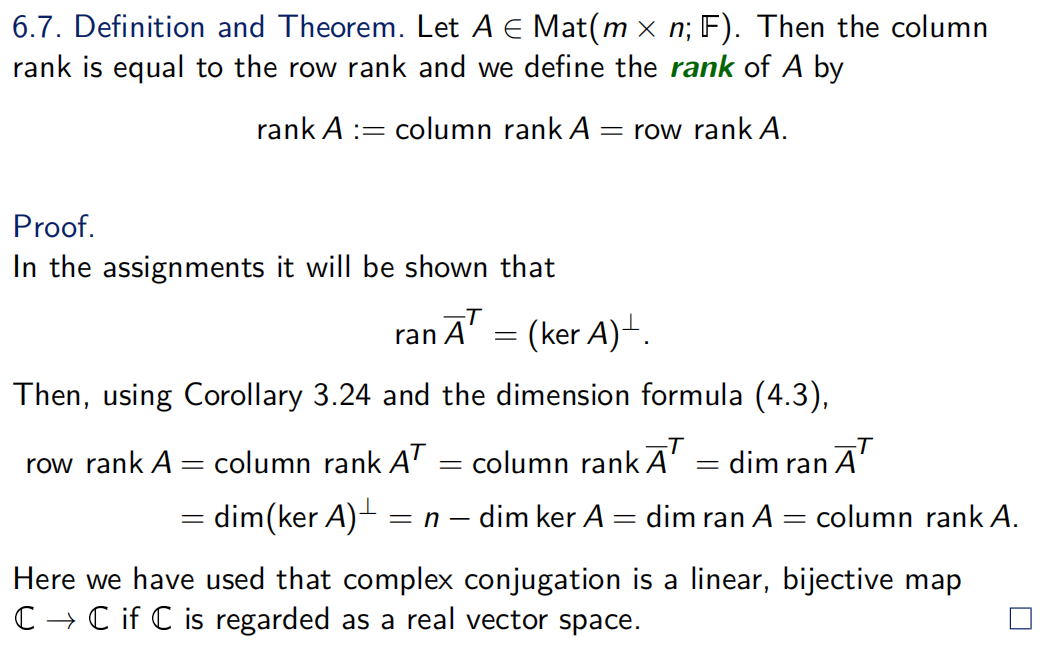
\includegraphics[width=\textwidth]{5}
    \end{center}
\end{frame}

\begin{frame}
    \frametitle{Systens of Equations}
    \begin{center}
        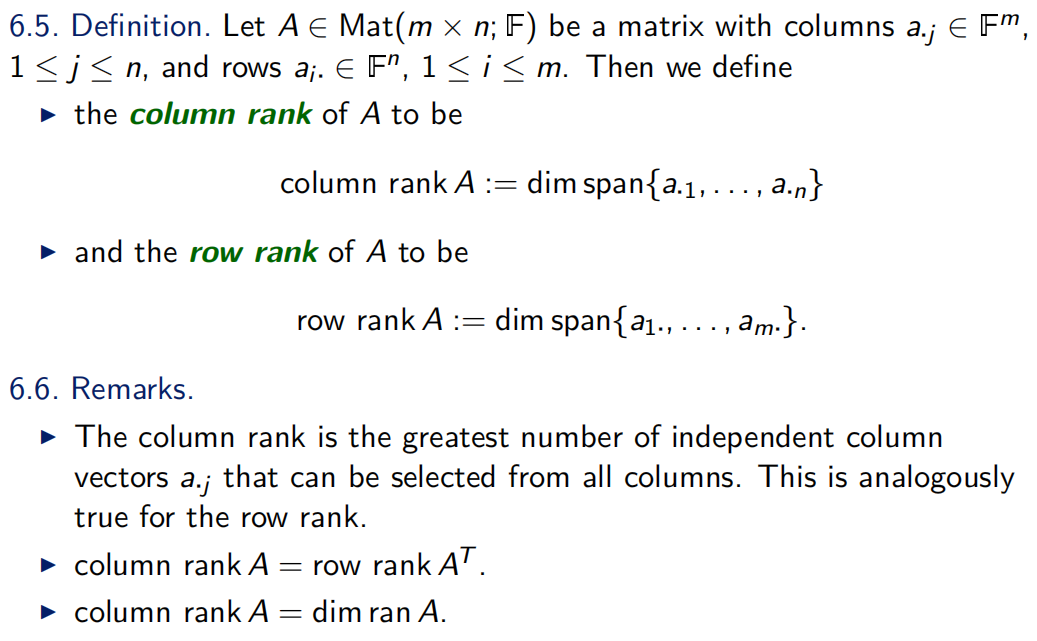
\includegraphics[width=\textwidth]{6}
    \end{center}
\end{frame}


\begin{frame}
    \frametitle{Deternimant}
    \begin{center}
        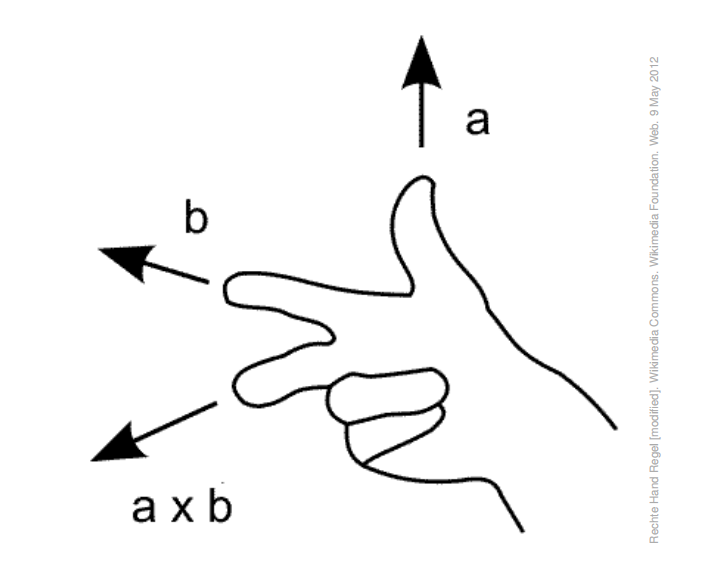
\includegraphics[width=0.8\textwidth]{8}
    \end{center}
\end{frame}


\begin{frame}
    \frametitle{Discussion}
    \vspace{1.5cm}
    \Large
    \centering
    Learn Well\\
    And\\
    Have Fun!\\


\end{frame}

\end{document}